\documentclass[UTF8]{EPURapport}
%\usepackage{listings}

%\renewcommand{\lstlistlistingname}{Liste des codes}
%\renewcommand{\lstlistingname}{Code}

%\addextratables{%
%	\lstlistoflistings
%}

%\swapAuthorsAndSupervisors

\thedocument{Rapport de projet}{Canne connectée pour aveugles}{}
\grade{Département Informatique\\ 5\ieme{} année\\ 2020-2021}
\authors{%
	\category{Auteurs}{%
		\name{Djawad M'DALLAH MARI} \mail{djawad.mdallah-mari@etu.univ-tours.fr}
	}
	\details{DII5 2020-2021}
}
\supervisors{%
	\category{Encadrants}{%
		\name{Gilles VENTURINI} \mail{gilles.venturini@etu.univ-tours.fr}
	}
	\details{Université François-Rabelais, Tours}
}
\abstracts{Rapport du projet canne connecée pour aveugles}
{}
{}
{}

\begin{document}

\chapter{Remerciements}

Premièrement, je voudrais adresser mes remerciements à mon encadrant de projet, \textbf{M. Gilles VENTURINI}, initiateur de ce projet. Ses conseils et recommandations m'ont permis de mener au mieux ce projet. En outre, je voudrais remercier l'ensemble de l'équipe pédagogique de \textbf{Polytech Tours}, pour leurs efforts et engagements durant ces périodes scolaires. Leurs efforts m'ont apporté connaissances et compétences indispensables que j'ai pu mettre en pratique durant la réalisation de ce projet. Je tiens également à remercier mes camarades pour leur soutien et leur collaboration durant ces années d'études. 

\chapter{Introduction}
Ce document est le rapport du projet intitulé "canne connectée pour aveugles" réalisé dans le cadre d'un projet de fin d'étude (PFE) à Polytech Tours. Elle vise à synthétiser le travail réalisé en montrant les différents aspects du projet tels que la gestion organisationnelle, technique et humaine.\\

Ce projet de fin d'étude est donc un projet qui vise à mettre en pratique les acquis de ces dernières années, en mettant en particulier un accent sur les capacités d'analyses et de réflexion ainsi que la rigueur des solutions proposées pour répondre aux problématiques.\\

Nous verrons donc dans ce document les problèmes posés, les enjeux associés et les réflexions menées pour aboutir à des solutions. Nous verrons dans un premier temps une présentation du projet ainsi que ces objectifs. Nous aborderons ensuite la stratégie d'approche servant d'axe principal pour mener ce projet. Après, nous verrons les méthodes et outils de gestion de projet qui ont été mis en place. Les choix et réalisations seront ensuite présentés suivi d'une prise de recul détaillant notamment les points critiques et les difficultés rencontrées lors du projet. Enfin, une conclusion sera faite apportant quelques remarques personnelles sur le projet.

\chapter{Présentation}

\section{Contexte}

Ce projet a été initié afin d'étudier les possibilités offertes par un smartphone pour pourvoir aider les malvoyants dans leur quotidien. En effet, il existe aujourd'hui plusieurs modèles de cannes connectées qui permettent d'aider les malvoyants à se déplacer. Ces cannes se basent sur différentes technologies (GPS, capteurs de mouvement, etc.) afin de renvoyer des informations utiles aux utilisateurs tels que la détection de chute ou encore la géolocalisation de l'individu.\\

Ce projet vise donc à enrichir ces informations transmis à l'utilisateur pour lui permettre de mieux percevoir leurs environnements. Pour cela, on souhaite donc explorer le potentiel des smartphones, ainsi que de l'intelligence artificielle (IA) afin de recueillir le maximum d'information sur un environnement donnée. Cela nous permettra de voir également les limites de l'intelligence artificielle employée dans ce cadre là.

\section{Objectifs}

L'objectif de ce PFE est de faire de la reconnaissance d'image à l'aide du smartphone. Plus précisément, faire de la reconnaissance d'objet en réalisant une application Android. Cette application devra permettre de reconnaître les objets du quotidien (bouteille, assiette, mug, etc.) ou d'autres objets sur un environnement plus large (poteau, trottoir, arbre, etc.).\\

L’application devra ensuite informer l’utilisateur de l’objet identifié. Cette information devra être indiquée à l’utilisateur d’une manière particulière, car l’application est destinée à des personnes malvoyantes. Pour cela, une étude des habitudes d'utilisation des personnes aveugles de leur smartphone sera nécessaire afin de déterminer le meilleur moyen de renvoyer ce type d'information.\\

Le périmètre de ce projet sera donc autour de cet objectif principal qui est donc de fournir un prototype d'une application Android renvoyant des informations utiles sur la scène qui entoure l'utilisateur. Par la suite, une extension du périmètre initial du projet pourra être envisagée afin d'intégrer ce système sur une canne pour aveugles. Cette intégration pourra se faire par l'ajout du smartphone directement sur la canne ou par la réalisation d'un boîtier avec des capteurs communiquant avec le smartphone.\\

Sur ce point, M.VENTURINI avait travaillé avec d'autres étudiants sur la faisabilité de ce projet sur un microcontrôleur et travail également avec des étudiants du département informatique (DI) sur l'enrichissement d'un réseau de neurones afin de pouvoir enregistrer et reconnaître des objets donnés.\\

Notre application sera donc un premier prototype qui nous permettra d'avoir un premier outil qu'on pourra présenter aux personnes malvoyantes afin d'avoir un retour précis sur leurs besoins. L’Institut d’éducation sensorielle pour sourds et aveugles IRECOV de Tours peut nous permettre d'entrer en contact avec des personnes aveugles afin de réaliser des tests.\\

\chapter{Motivation et stratégie d'approche}

\section{Motivations}

J'ai été particulièrement intéressé par ce projet, car c'était une occasion pour moi de découvrir le domaine de l'intelligence artificielle et des réseaux de neurones. En effet, durant mes années d'études, je n'ai pas eu l'occasion de suivre des cours là-dessus ni de travailler sur des projets mettant en œuvre ce type de technique. Ceci, malgré qu'on en entend de plus en plus dans différents domaines d'application. Il me semblait donc intéressant de saisir cette occasion afin de m'initier et comprendre quelques mécanismes sur son fonctionnement.\\

J'ai aussi été attiré par le fait que ce travail pourrait servir concrètement à des personnes réelles et n'est donc pas qu'un simple projet académique permettant de mettre en œuvre les acquis. Un réel besoin existe auprès des utilisateurs finaux, ce qui motive fortement à être engagé afin de faire aboutir ce projet.\\

Un autre point est que, malgré le fait que je n'ai pas eu l'occasion de suivre des cours sur de l'intelligence artificielle ou le fonctionnement des réseaux de neurones, j'ai déjà de l'expérience dans la réalisation d'application Android. En effet, j'ai pu réaliser une application Android durant mon stage de DUT, et ça m'a permis non seulement de renforcer mes compétences en Java, mais aussi de découvrir le monde du développement mobile. L'aspect technique de ce projet n'est donc pas un frein pour moi, mais plutôt elle me permettra de me baser sur mes acquis afin d'appréhender l'intelligence artificielle sereinement.\\

Ce projet est donc un challenge qui me permettra de consolider mes acquis et d'élargir mes compétences et connaissances sur d'autres facettes de l'informatique.

\section{Stratégie d'approche}

Les enjeux du projet de fin d'études n'étant pas tournés autour de la technique, j'ai préféré me concentrer sur d'autres points tout aussi important dans ce type de projet. En effet, pour qu'un projet soit réussi, il faut être capable de prendre du recul et gérer les autres aspects autour de la technique telle que \textbf{la gestion du projet} au sens organisationnel, \textbf{anticiper les risques} et \textbf{respecter les délais et le budget}. Une de mes stratégies fut donc la mise en place de planning afin d'organiser chaque phase du projet du début à la fin.\\

Il faut également \textbf{être à l'écoute du client}. C'est pourquoi mettre en place une bonne \textbf{communication avec le client} est essentiel, car cela permettra de bien comprendre le besoin et donc d'être capable de fournir des solutions adéquates. Cette communication régulière permet également de faire un point sur l'avancement du projet et de valider les fonctionnalités implémentées. C'est donc une des stratégies que j'ai pu mettre en place avec le client de manière hebdomadaire par appel ou par mail.\\

Un point important est aussi le fait de fournir un travail qui pourra être repris facilement à la fin du projet. L'importance apportée aux livrables sur le projet de cette année permet donc de fournir des documents qui réunissent tous les éléments nécessaires à \textbf{la reprise du projet}. Ce rapport sera donc accompagné du cahier de spécification, le cahier d'analyse, le manuel développeur, le manuel mainteneur, le manuel administrateur ainsi que le manuel utilisateur. Ces documents faciliteront donc la reprise du projet. J'ai également commenté les parties les plus importantes du code source du projet, mais aussi essayer de respecter les normes de codage et les bonnes pratiques. Tout ceci sur mon github \footnote{ Code source: \url{https://github.com/Djawad-mdallahmari/PFE-ObjectDetection} \\ Documentation: \url{https://github.com/Djawad-mdallahmari/PFE-Documentation}} avec l'historique depuis le début du projet afin de pouvoir revenir sur d'anciennes versions si besoin.

\chapter{Gestion du projet}

\section{Plannings}

Parmi les éléments qui m'ont aidé à gérer mon temps, il y a le planning prévisionnel que j'ai établi en début de projet. Ce planning m'a permis de définir clairement chaque phase du projet et de leur attribuer un temps limité. Ceci, m'a donc forcé à respecter les délais que je me suis attribués pour chaque phase ainsi que les jalons prévus par Polytech sur les différents livrables à rendre. \\

\begin{figure}[h!]
\centering
  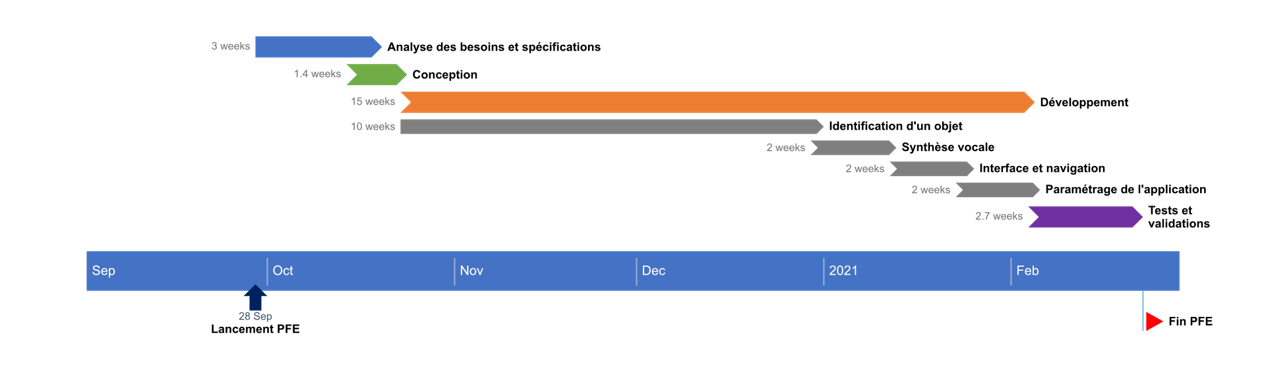
\includegraphics[width=\textwidth]{images/PlanningPrev.png}
  \caption{Planning prévisionnel}
  \label{fig:planningprev}
\end{figure}

Dans ce planning, j'ai décidé de rester assez général en indiquant seulement les grandes phases du projet sans détailler chaque tâche que j'allais faire. Ceci pour deux raisons : 

\begin{itemize}
  \item La première est le fait qu'à ce stade du projet, il est encore difficile d'imaginer chaque tâche et fonctionnalités que je serai amené à faire. En effet, au début du projet, il a fallu que j'étudie le besoin du client et ensuite faire une analyse de ces besoins afin de pouvoir proposer des solutions.
  \item La deuxième est que la définition de chaque tâche à faire en début du projet se traduira par une spécification figée qu'on ne pourra changer selon l'avancé du projet. Ce qui est une des inconvénients du cycle en V. J'ai donc voulu allier la méthode cycle en V en réutilisant ses différentes phases de projet tout en prenant quelques concepts du modèle agile en y introduisant une souplesse dans les spécifications ainsi que dans les tâches que je serai amené à réaliser.
\end{itemize}

En procédant ainsi, j'ai décidé de ne détailler que la phase de développement en y ajoutant les fonctionnalités que je devais implémenter et le temps que cela me prendrait (éléments en gris sur le planning).\\

Sur ce planning, j'ai décidé de ne pas représenter les tâches liées aux livrables. Ces tâches seront réalisées en parallèle des différentes phases du projet. Lors de la phase d'analyse et de spécification des besoins, j'ai rédigé en parallèle le cahier de spécification puis le cahier d'analyse. De même pour le rapport et les autres livrables qui seront rédigé vers la fin du projet. Cependant, il y a quelques écarts entre le planning prévisionnel et le planning réel. \\

\begin{figure}[h!]
\centering
  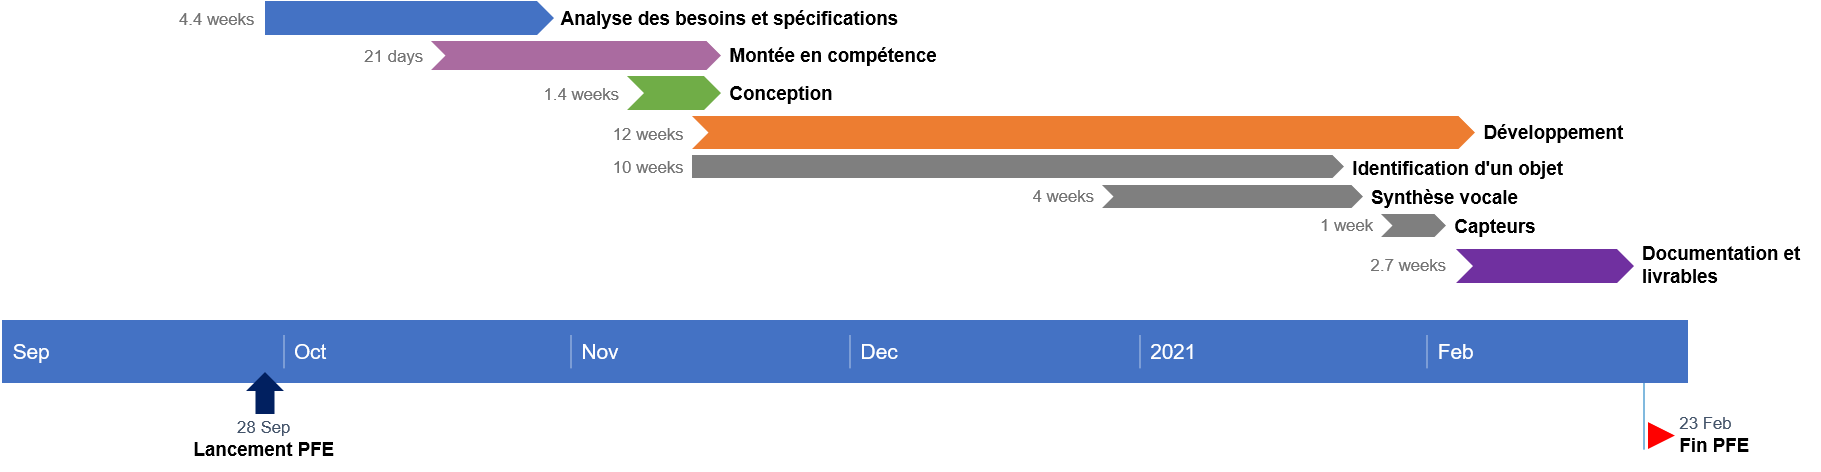
\includegraphics[width=\textwidth]{images/PlanningReel.png}
  \caption{Planning réel}
  \label{fig:planningreel}
\end{figure}

Dans le planning réel, la phase d'analyse a duré plus longtemps que prévu, car il a fallu que je monte en compétences afin de comprendre comment fonctionne l'intelligence artificielle, les technologies à utiliser pour l'implémenter, étudier les avantages et inconvénients de chacun etc. avant d'être capable de proposer une solution. J'ai donc empiéter sur la phase de développement, mais j'ai quand même commencé à regarder quelques codes très tôt et de les modifier afin de comprendre comment cela fonctionnait. \\

Ensuite, on remarque que certaines fonctionnalités comme la réalisation d'une interface de navigation a été omis. Ceci car en fonction de l'avancée du projet, on a remarqué cela n'était pas forcément utile puisque l'utilisateur n'a pas besoin d'accéder à d'autres menus. Dans notre application il y a qu'une barre qu'on peut faire apparaître afin de faire quelques réglages, mais l'utilisateur dans un premier temps n'aura pas besoin de régler ces paramètres-là pour utiliser l'application. \\

Cette modification est donc le résultat d'un suivi régulier qui a permis de déterminer ce qui est important de ce qui l'est moins. Nous avons donc utilisé ce temps afin de réfléchir à d'autres fonctionnalités qui pourraient nous être utiles comme la mise en place de différents capteurs. Dans l'optique de fournir à l'utilisateur un maximum d'informations sur un environnement donné, l'utilisation de ces informations venant des capteurs pourraient donc nous être plus utile que de réaliser une interface de navigation. 

\section{Gestion des tâches}

Pour la gestion des tâches de manière plus minutieuse, j'ai décidé de mettre en place un \textbf{Trello}. \\

\begin{figure}[h!]
\centering
  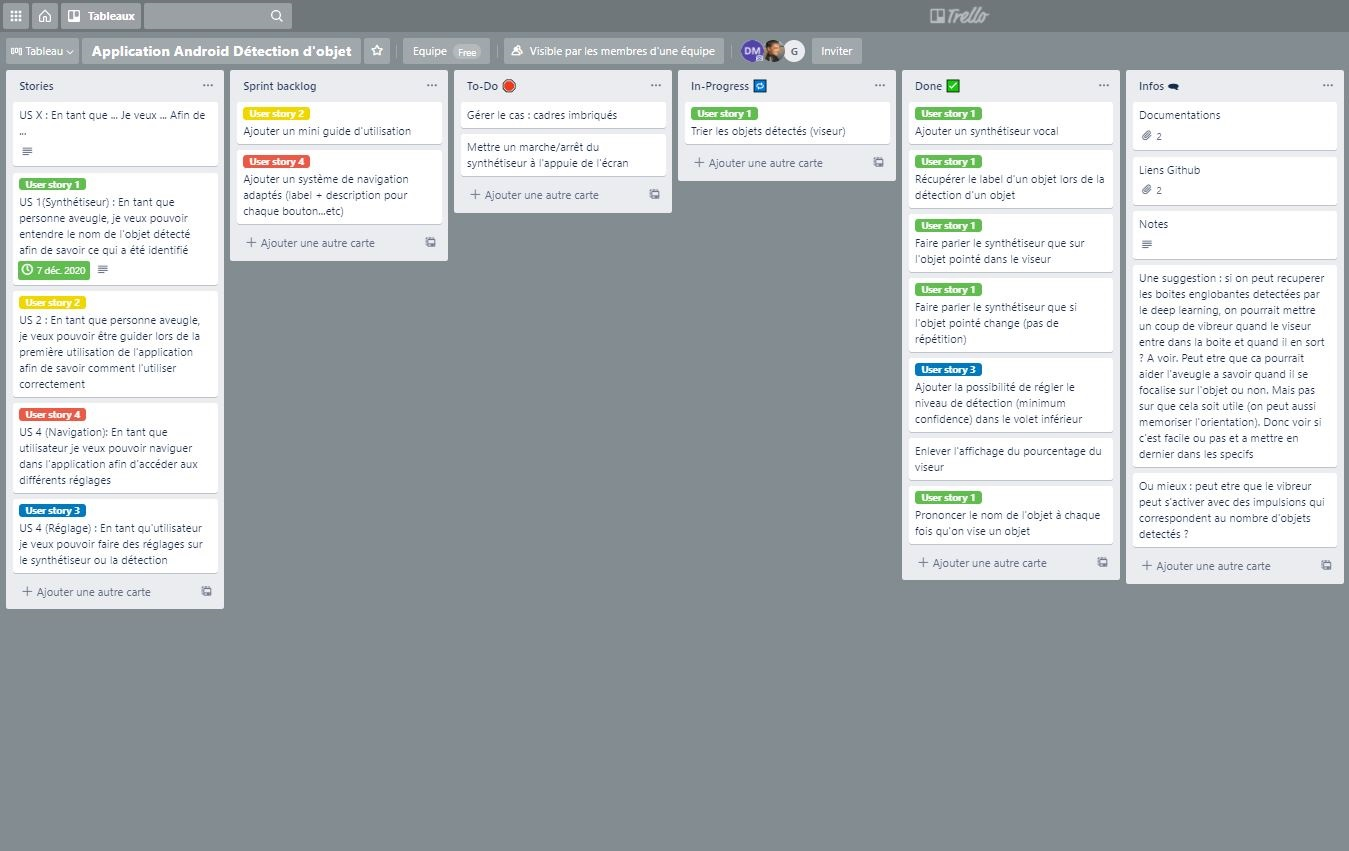
\includegraphics[width=\textwidth]{images/Trello1.JPG}
  \caption{Exemple état du Trello en phase développement}
  \label{fig:trello}
\end{figure}

Ce Trello m'a permis d'avoir une vue globale des tâches qui ont été faites et ceux qui restent à faire. J'ai décidé de l'organiser un peu à la manière des tableaux des méthodologies agiles puisque je venais le mettre à jour à la fin de nos réunions hebdomadaires avec le client. Cela permettait donc de valider ce qui avait été fait mais aussi de noter ce qui est à faire pour la prochaine réunion à la manière des sprints dans la méthodologie Scrum. De cette manière, je gardais donc une flexibilité sur les tâches à faire en fonction des retours du client tout en gardant un suivi sur la fonctionnalité auquel chaque tâche est liée. En effet, chaque tâche devait être liée à une fonctionnalité donnée qui répond à un besoin du client/utilisateur. C'est pour cela que j'ai décidé de décrire les fonctionnalités sous forme de User Story. En faisant ainsi, on comprend le besoin et le pourquoi de chaque tâche.\\

Cependant, un autre point que j'ai volontairement décidé de ne pas utiliser sur Trello est l'attribution d'une date butoir à chaque tâche ainsi que l'attribution d'une tâche à chacune des parties prenantes du projet. En effet, je partais de l'idée que les tâches les plus prioritaires sont ceux qui ont été discuté lors de la précédente réunion, je les passe donc dans la colonne "To Do" sans déterminer la date butoir ni prendre la peine de déterminer la personne qui devait la faire puisque ça allait forcément être moi-même. Ce point aurait été plus intéressant dans le cadre d'une équipe plus large avec plusieurs développeurs par exemple. \\

Je me suis donc inspiré de la méthode agile sur l'établissement de ce Trello sans pour autant être stricte sur les concepts de la méthode tel que l'établissement d'un backlog ou la production d'un MVP (Minimum Viable Product) à la fin de chaque sprint. 

\section{Versionning}

Afin d'avoir un suivi de chaque changement, que ce soit au niveau des documents ou au niveau du programme, j'ai utilisé \textbf{Git} dès le départ. Pour les documents, chaque version est écrite dans la première page du document (sauf la version finale). Cela permet donc de revenir à une ancienne version d'un document en ayant la date de la dernière modification.\\

Le git me permet également de stocker les différentes versions de tests de l'application (les .apk) que je déploie afin que le client puisse tester les nouvelles fonctionnalités implémentées. Ainsi, on garde un état de l'application après chaque déploiement. Si on souhaite déployer une nouvelle version de l'application sur le Google Play par exemple, ce système nous permet de revenir à la version précédente en cas de bug non identifié, mais remonté par les utilisateurs.\\

C'est donc un bon moyen de fournir l'ensemble du projet avec son historique afin que le projet soit repris facilement dans son entièreté \footnote{Attention, le github est sur mon compte étudiant et risque peut-être de disparaître lorsque mon compte étudiant ne sera plus valide. En cas de reprise du projet, il faudra veiller à cloner ces repository rapidement dès le départ.}.

\chapter{Choix et réalisations}

\section{Framework et modèle}

Pour répondre au \textbf{besoin d'identification d'un objet}, j'ai choisi d'utiliser la librairie \textbf{TensorFlow Lite}. C'est la librairie la plus commune et la plus adaptée pour faire de l'intelligence artificielle sur mobile, comme cela a été vu dans le cahier d'analyse.\\

TensorFlow Lite est une librairie qui permet d'utiliser des modèles de réseau de neurones préentrainés. Il existe différents types de modèles en fonction de ce que l'on souhaite faire. Dans notre cas, il s'agit de faire de la détection d'objet. Il faut donc choisir un modèle qui nous convient qui permet de faire cela. Pour cela, j'ai choisi le modèle \textbf{MobileNetV2}. Ce choix a été fait suite à l'analyse des possibilités existantes que vous pouvez retrouver dans le cahier d'analyse. En résumé, ce modèle utilise une architecture adaptée pour le mobile et pour les matériels ayant peu de ressources. Cette architecture réduit le nombre d'opérations \footnote{Opérations Tensorflow Lite : \url{https://www.tensorflow.org/mlir/tfl_ops}} et réduit la consommation de la mémoire tout en gardant la même précision. Ce modèle a été entraîné avec les images de COCO dataset \footnote{\url{https://cocodataset.org/}}. Ses résultats lors de mon bunchmark ont été satisfaisant et donc l'utilisation de ce modèle est suffisant pour répondre à notre besoin.

\section{Intégration du modèle}

Pour utiliser ce modèle, je ne suis pas parti d'une application Android que j'ai créée à partir de zéro. Je préférais me baser directement sur l'exemple fourni par Tensorflow sur leur github \footnote{\url{https://github.com/tensorflow}}. Cela me permet de gagner beaucoup de temps et d'avoir une base solide pour implémenter les autres fonctionnalités. L'exemple vient avec deux méthodes d'intégration du modèle qu'on peut choisir au moment de builder l'application : TensorFlow Lite Task Library \footnote{\url{https://www.tensorflow.org/lite/inference_with_metadata/task_library/object_detector}} et TensorFlow Lite Interpreter API \footnote{\url{https://www.tensorflow.org/lite/guide/inference}}. Ces deux librairies permettent d'intégrer à l'application Android le modèle, mais surtout de l'interpréter. Une fois que ces librairies auront été ajoutées grâce aux gestionnaires de dépendance Gradle, Android Studio nous permet de choisir un des deux à utiliser pour builder l'application.\\

Ensuite, pour reconnaître des objets sur une image, il suffit (après toutes les étapes d'initialisations) d'appeler la méthode \verb|recognizeImage(Bitmap bitmap)| qui nous renvoie un ensemble de résultats. Ces résultats sont retournés au sein d'un objet contenant un id, un titre, un taux de confiance et la localisation de l'objet.

\section{Synthétiseur vocal}

\section{Viseur virtuel}

\section{Start and Stop}

\section{Capteurs}

\section{Documentations}

\chapter{Prise de recul}

\section{Points positifs}

\section{Points critiques}

\section{Difficultés}

\section{Améliorations possibles}

\chapter{Conclusion}

\annexes

\end{document}